\section{Herramientas, estilos y estructuras en programación paralela}\label{herramientas-progpar}

\subsection{Problemas que plantea la programación paralela al programador}\label{problemas-progpar}

La programación paralela plantea problemas inherentes a la misma que no se dan en la programación secuencial, como la división del cómputo total en tareas independientes, la agrupación de dichas tareas en procesos o hebras, la asignación de estos procesos y hebras a los procesadores y la sincronización y comunicación entre estos procesos.
Estos problemas deben ser abordados tanto por la herramienta de programación como por el programador.

Para escribir un programa de forma paralela partimos de su versión secuencial y lo dividimos en bloques sin dependencias de datos.
También podemos utilizar versiones optimizadas para la programación paralela de las bibliotecas que importemos.

Al trabajar con programación paralela en arquitecturas MIMD podemos hacerlo de forma \textbf{SPMD}, paralelizando un solo programa, (\textit{Single Program Multiple Data}) y \textbf{MPMD} (\textit{Multiple Program Multiple Data}), paralelizando la ejecución de varios programas que a su vez están programados de forma paralela.

\subsection{Herramientas para obtener código paralelo}\label{herramientas-codigo-par}

Para crear programas de ejecución paralela podemos utilizar las tres técnicas ordenadas de menor a mayor abstracción:

\begin{itemize}
	\item\textbf{Compiladores paralelos:} Extraen automáticamente el paralelismo de los programas que compilan, de forma que el programador no tiene que explicitarla.
	\item\textbf{Lenguajes paralelos y API de directivas:} La sintáxis de los lenguajes paralelos como Occam, Ada o Haskell o las directivas de OpenMP permiten indicar cómo paralelizar el programa en el código a gusto del programador.
	\item\textbf{API de funciones:} Las APIs de alto nivel como OpenMPI permiten paralelizar la programación mediante paso de mensajes y otras técnicas de abstracción alta.
\end{itemize}

Las herramientas de paralelización permiten, implícita o explícitamente, localizar el paralelismo de los programas dividiéndolos en tareas independientes, asignar tareas a los procesos y hebras, crear y terminar estos procesos y hebras y comunicarlos y sincronizarlos.
El \textbf{\textit{mapping}}, la asignación de las diferentes tareas a procesos y threads, puede hacerlo el programador, la herramienta de programación paralela o el propio sistema operativo.

\pagebreak

Por ejemplo, así se haría un cálculo de el número $\pi$ con OpenMP\@:

\begin{lstlisting}[language=C]
#include <opm.h>
#include <stdlib.h>
#define NUM_THREADS 4

int main (int argc, char ** argv) {
	double ancho,
	       sum = 0,
	       x;
	int intervalos;

	intervalos = atoi(argv[1]);
	ancho      = 1.0 / (double) intervalos;

	omp_set_num_threads(NUM_THREADS);

	#pragma omp parallel
	{
		#pragma omp for reduction(+:sum) private(x) schedule(dynamic)
		for (int i=0; i<intervalos; i++) {
			x    = (i + 0.5) * ancho;
			sum += 4.0 / (1.0 + x * x);
		}
	}

	sum *= ancho;
}
\end{lstlisting}

Y así se haría el mismo cómputo con MPI\@:

\begin{lstlisting}[language=C]
#include <mpi.h>
#include <stdlib.h>

int main (int argc, char ** argv) {
	double ancho,
	       lsum,
	       sum = 0,
	       x;
	int intervalos
	    iproc,
	    nproc;

	if (MPI_Init(&argc, &argv) != MPI_SUCCESS)
		exit (1);

	MPI_Comm_size(MPI_COMM_WORLD, &nproc);
	MPI_Comm_rank(MPI_COMM_WORLD, &iproc);

	intervalos = atoi(argv[1]);
	ancho = 1.0 / (double) intervalos;

	for (int i=iproc; i<intervalos; i=nproc) {
		x = (i + 0.5) * ancho;
		sum += 4.0 / (1.0 + x * x);
	}

	lsum *= ancho;

	MPI_Reduce(&lsum, &sum, 1, MPI_DOUBLE, MPI_SUM, 0, MPI_COMM_WORLD);

	MPI_Finalize();
}
\end{lstlisting}

\subsubsection{Comunicaciones colectivas}

Distinguimos entre diferentes tipos de comunicaciones entre procesos y hebras:

\textbf{Comunicación \textit{uno a todos}}

Se caracterizan porque un único proceso envía un mensaje a varios procesos al mismo tiempo.
Esto puede conseguirse mediante una \textbf{difusión} (\textit{broadcast}) del mensaje, que envía un mensaje $x$ a todos los procesos a la vez, o mediante una \textbf{dispersión} (\textit{scatter}), que envía envía un mensaje $x_i$ a cada proceso $i$.

\begin{figure}[h]
\begin{center}
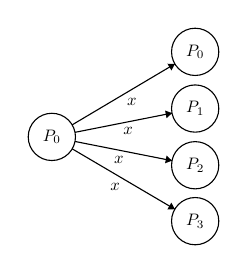
\begin{tikzpicture}[scale=0.1, every node/.style={scale=0.6}]
\tikzstyle{every node}+=[inner sep=0pt]
\draw [black] (3.2,-14) circle (3);
\draw (3.2,-14) node {$P_0$};
\draw [black] (21.4,-3.2) circle (3);
\draw (21.4,-3.2) node {$P_0$};
\draw [black] (21.4,-10.4) circle (3);
\draw (21.4,-10.4) node {$P_1$};
\draw [black] (21.4,-17.6) circle (3);
\draw (21.4,-17.6) node {$P_2$};
\draw [black] (21.4,-24.7) circle (3);
\draw (21.4,-24.7) node {$P_3$};
\draw [black] (6.14,-13.42) -- (18.46,-10.98);
\fill [black] (18.46,-10.98) -- (17.58,-10.65) -- (17.77,-11.63);
\draw (12.89,-12.79) node [below] {$x$};
\draw [black] (6.14,-14.58) -- (18.46,-17.02);
\fill [black] (18.46,-17.02) -- (17.77,-16.37) -- (17.58,-17.35);
\draw (11.71,-16.39) node [below] {$x$};
\draw [black] (5.79,-15.52) -- (18.81,-23.18);
\fill [black] (18.81,-23.18) -- (18.38,-22.34) -- (17.87,-23.21);
\draw (11.24,-19.85) node [below] {$x$};
\draw [black] (5.78,-12.47) -- (18.82,-4.73);
\fill [black] (18.82,-4.73) -- (17.88,-4.71) -- (18.39,-5.57);
\draw (13.36,-9.1) node [below] {$x$};
\end{tikzpicture}

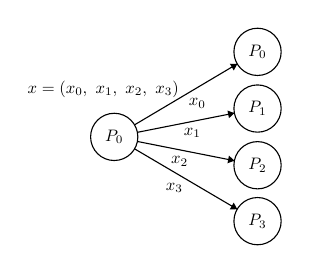
\begin{tikzpicture}[scale=0.1, every node/.style={scale=0.6}]
\tikzstyle{every node}+=[inner sep=0pt]
\draw [black] (8.4,-14) circle (3);
\draw (8.4,-14) node {$P_0$};
\draw [black] (26.6,-3.2) circle (3);
\draw (26.6,-3.2) node {$P_0$};
\draw [black] (26.6,-10.4) circle (3);
\draw (26.6,-10.4) node {$P_1$};
\draw [black] (26.6,-17.6) circle (3);
\draw (26.6,-17.6) node {$P_2$};
\draw [black] (26.6,-24.7) circle (3);
\draw (26.6,-24.7) node {$P_3$};
\draw (7,-7.9) node {$x=(x_0,\mbox{ }x_1,\mbox{ }x_2,\mbox{ }x_3)$};
\draw [black] (11.34,-13.42) -- (23.66,-10.98);
\fill [black] (23.66,-10.98) -- (22.78,-10.65) -- (22.97,-11.63);
\draw (18.31,-12.83) node [below] {$x_1$};
\draw [black] (11.34,-14.58) -- (23.66,-17.02);
\fill [black] (23.66,-17.02) -- (22.97,-16.37) -- (22.78,-17.35);
\draw (16.69,-16.43) node [below] {$x_2$};
\draw [black] (10.99,-15.52) -- (24.01,-23.18);
\fill [black] (24.01,-23.18) -- (23.58,-22.34) -- (23.07,-23.21);
\draw (16.04,-19.85) node [below] {$x_3$};
\draw [black] (10.98,-12.47) -- (24.02,-4.73);
\fill [black] (24.02,-4.73) -- (23.08,-4.71) -- (23.59,-5.57);
\draw (18.96,-9.1) node [below] {$x_0$};
\end{tikzpicture}

\end{center}
\caption{Difusión y dispersión de mensajes}
\end{figure}

\textbf{Comunicación \textit{todos a uno}}

Se caracterizan porque un único proceso recibe un mensaje a partir de los mensajes enviados por varios procesos.
Esta recepción puede hacerse mediante \textbf{reducción} cuando los mensajes recibidos son argumentos de una función o mediante \textbf{acumulación} (\textit{gather}), cuando se recogen indistintamente todos los mensajes.

\begin{figure}[h]
\begin{center}
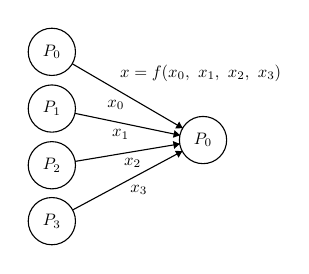
\begin{tikzpicture}[scale=0.1, every node/.style={scale=0.6}]
\tikzstyle{every node}+=[inner sep=0pt]
\draw [black] (22.4,-14.4) circle (3);
\draw (22.4,-14.4) node {$P_0$};
\draw [black] (3.2,-3.2) circle (3);
\draw (3.2,-3.2) node {$P_0$};
\draw [black] (3.2,-10.4) circle (3);
\draw (3.2,-10.4) node {$P_1$};
\draw [black] (3.2,-17.6) circle (3);
\draw (3.2,-17.6) node {$P_2$};
\draw [black] (3.2,-24.7) circle (3);
\draw (3.2,-24.7) node {$P_3$};
\draw (22.1,-5.9) node {$x=f(x_0,\mbox{ }x_1,\mbox{ }x_2,\mbox{ }x_3)$};
\draw [black] (6.14,-11.01) -- (19.46,-13.79);
\fill [black] (19.46,-13.79) -- (18.78,-13.14) -- (18.58,-14.11);
\draw (11.94,-13.03) node [below] {$x_1$};
\draw [black] (5.79,-4.71) -- (19.81,-12.89);
\fill [black] (19.81,-12.89) -- (19.37,-12.05) -- (18.87,-12.92);
\draw (11.34,-9.3) node [below] {$x_0$};
\draw [black] (6.16,-17.11) -- (19.44,-14.89);
\fill [black] (19.44,-14.89) -- (18.57,-14.53) -- (18.73,-15.52);
\draw (13.44,-16.64) node [below] {$x_2$};
\draw [black] (5.84,-23.28) -- (19.76,-15.82);
\fill [black] (19.76,-15.82) -- (18.82,-15.76) -- (19.29,-16.64);
\draw (14.26,-20.05) node [below] {$x_3$};
\end{tikzpicture}

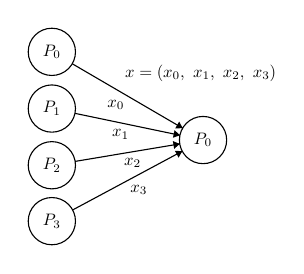
\begin{tikzpicture}[scale=0.1, every node/.style={scale=0.6}]
\tikzstyle{every node}+=[inner sep=0pt]
\draw [black] (22.4,-14.4) circle (3);
\draw (22.4,-14.4) node {$P_0$};
\draw [black] (3.2,-3.2) circle (3);
\draw (3.2,-3.2) node {$P_0$};
\draw [black] (3.2,-10.4) circle (3);
\draw (3.2,-10.4) node {$P_1$};
\draw [black] (3.2,-17.6) circle (3);
\draw (3.2,-17.6) node {$P_2$};
\draw [black] (3.2,-24.7) circle (3);
\draw (3.2,-24.7) node {$P_3$};
\draw (22.1,-5.9) node {$x=(x_0,\mbox{ }x_1,\mbox{ }x_2,\mbox{ }x_3)$};
\draw [black] (6.14,-11.01) -- (19.46,-13.79);
\fill [black] (19.46,-13.79) -- (18.78,-13.14) -- (18.58,-14.11);
\draw (11.94,-13.03) node [below] {$x_1$};
\draw [black] (5.79,-4.71) -- (19.81,-12.89);
\fill [black] (19.81,-12.89) -- (19.37,-12.05) -- (18.87,-12.92);
\draw (11.34,-9.3) node [below] {$x_0$};
\draw [black] (6.16,-17.11) -- (19.44,-14.89);
\fill [black] (19.44,-14.89) -- (18.57,-14.53) -- (18.73,-15.52);
\draw (13.44,-16.64) node [below] {$x_2$};
\draw [black] (5.84,-23.28) -- (19.76,-15.82);
\fill [black] (19.76,-15.82) -- (18.82,-15.76) -- (19.29,-16.64);
\draw (14.26,-20.05) node [below] {$x_3$};
\end{tikzpicture}

\end{center}
\caption{Reducción y acumulación de mensajes}
\end{figure}

\textbf{Comunicación \textit{todos a todos}}

En este tipo de comunicación todos los procesos se comunican con todos.
Esto se puede hacer mediante un sistema en el que \textbf{todos difunden} (\textit{all-broadcast}), también conocido como chismorreo (\textit{gossiping}), o mediante un sistema en el que \textbf{todos dispersan} (\textit{all-scatter}).

\begin{figure}[h]
\begin{center}
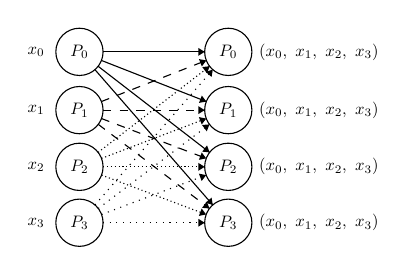
\begin{tikzpicture}[scale=0.1, every node/.style={scale=0.6}]
\tikzstyle{every node}+=[inner sep=0pt]
\draw [black] (25.5,-3.2) circle (3);
\draw (25.5,-3.2) node {$P_0$};
\draw [black] (6.6,-3.2) circle (3);
\draw (6.6,-3.2) node {$P_0$};
\draw [black] (6.6,-17.8) circle (3);
\draw (6.6,-17.8) node {$P_2$};
\draw [black] (6.6,-24.9) circle (3);
\draw (6.6,-24.9) node {$P_3$};
\draw (37,-3.2) node {$(x_0,\mbox{ }x_1,\mbox{ }x_2,\mbox{ }x_3)$};
\draw [black] (25.5,-10.6) circle (3);
\draw (25.5,-10.6) node {$P_1$};
\draw [black] (25.5,-17.8) circle (3);
\draw (25.5,-17.8) node {$P_2$};
\draw [black] (25.5,-24.9) circle (3);
\draw (25.5,-24.9) node {$P_3$};
\draw [black] (6.6,-10.6) circle (3);
\draw (6.6,-10.6) node {$P_1$};
\draw (37,-10.6) node {$(x_0,\mbox{ }x_1,\mbox{ }x_2,\mbox{ }x_3)$};
\draw (37,-17.8) node {$(x_0,\mbox{ }x_1,\mbox{ }x_2,\mbox{ }x_3)$};
\draw (37,-24.9) node {$(x_0,\mbox{ }x_1,\mbox{ }x_2,\mbox{ }x_3)$};
\draw (1.1,-3.2) node {$x_0$};
\draw (1.1,-10.6) node {$x_1$};
\draw (1.1,-17.8) node {$x_2$};
\draw (1.1,-24.9) node {$x_3$};
\draw [black] (9.6,-3.2) -- (22.5,-3.2);
\fill [black] (22.5,-3.2) -- (21.7,-2.7) -- (21.7,-3.7);
\draw [black] [densely dotted] (8.97,-15.97) -- (23.13,-5.03);
\fill [black] (23.13,-5.03) -- (22.19,-5.13) -- (22.8,-5.92);
\draw [black] [dotted] (8.57,-22.64) -- (23.53,-5.46);
\fill [black] (23.53,-5.46) -- (22.63,-5.74) -- (23.38,-6.39);
\draw [black] (9.39,-4.29) -- (22.71,-9.51);
\fill [black] (22.71,-9.51) -- (22.14,-8.75) -- (21.78,-9.68);
\draw [black] (8.97,-5.03) -- (23.13,-15.97);
\fill [black] (23.13,-15.97) -- (22.8,-15.08) -- (22.19,-15.87);
\draw [black] (8.57,-5.46) -- (23.53,-22.64);
\fill [black] (23.53,-22.64) -- (23.38,-21.71) -- (22.63,-22.36);
\draw [black] [dashed] (9.39,-9.51) -- (22.71,-4.29);
\fill [black] (22.71,-4.29) -- (21.78,-4.12) -- (22.14,-5.05);
\draw [black] [dashed] (9.6,-10.6) -- (22.5,-10.6);
\fill [black] (22.5,-10.6) -- (21.7,-10.1) -- (21.7,-11.1);
\draw [black] [dashed] (9.4,-11.67) -- (22.7,-16.73);
\fill [black] (22.7,-16.73) -- (22.13,-15.98) -- (21.77,-16.91);
\draw [black] [dashed] (8.99,-12.41) -- (23.11,-23.09);
\fill [black] (23.11,-23.09) -- (22.77,-22.21) -- (22.17,-23.01);
\draw [black] [densely dotted] (9.4,-16.73) -- (22.7,-11.67);
\fill [black] (22.7,-11.67) -- (21.77,-11.49) -- (22.13,-12.42);
\draw [black] [densely dotted] (9.6,-17.8) -- (22.5,-17.8);
\fill [black] (22.5,-17.8) -- (21.7,-17.3) -- (21.7,-18.3);
\draw [black] [densely dotted] (9.41,-18.85) -- (22.69,-23.85);
\fill [black] (22.69,-23.85) -- (22.12,-23.1) -- (21.77,-24.03);
\draw [black] [dotted] (8.99,-23.09) -- (23.11,-12.41);
\fill [black] (23.11,-12.41) -- (22.17,-12.49) -- (22.77,-13.29);
\draw [black] [dotted] (9.41,-23.85) -- (22.69,-18.85);
\fill [black] (22.69,-18.85) -- (21.77,-18.67) -- (22.12,-19.6);
\draw [black] [dotted] (9.6,-24.9) -- (22.5,-24.9);
\fill [black] (22.5,-24.9) -- (21.7,-24.4) -- (21.7,-25.4);
\end{tikzpicture}

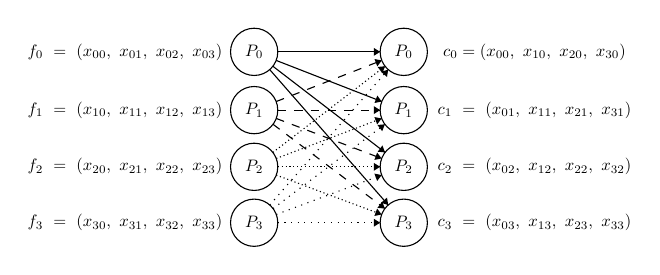
\begin{tikzpicture}[scale=0.1, every node/.style={scale=0.6}]
\tikzstyle{every node}+=[inner sep=0pt]
\draw [black] (41.4,-3.2) circle (3);
\draw (41.4,-3.2) node {$P_0$};
\draw [black] (22.4,-3.2) circle (3);
\draw (22.4,-3.2) node {$P_0$};
\draw [black] (22.4,-17.8) circle (3);
\draw (22.4,-17.8) node {$P_2$};
\draw [black] (22.4,-24.9) circle (3);
\draw (22.4,-24.9) node {$P_3$};
\draw (58,-3.2) node {$c_0=(x_{00},\mbox{ }x_{10},\mbox{ }x_{20},\mbox{ }x_{30})$};
\draw [black] (41.4,-10.6) circle (3);
\draw (41.4,-10.6) node {$P_1$};
\draw [black] (41.4,-17.8) circle (3);
\draw (41.4,-17.8) node {$P_2$};
\draw [black] (41.4,-24.9) circle (3);
\draw (41.4,-24.9) node {$P_3$};
\draw [black] (22.4,-10.6) circle (3);
\draw (22.4,-10.6) node {$P_1$};
\draw (58,-10.6) node {$c_1\mbox{ }=\mbox{ }(x_{01},\mbox{ }x_{11},\mbox{ }x_{21},\mbox{ }x_{31})$};
\draw (58,-17.8) node {$c_2\mbox{ }=\mbox{ }(x_{02},\mbox{ }x_{12},\mbox{ }x_{22},\mbox{ }x_{32})$};
\draw (58,-24.9) node {$c_3\mbox{ }=\mbox{ }(x_{03},\mbox{ }x_{13},\mbox{ }x_{23},\mbox{ }x_{33})$};
\draw (6,-3.2) node {$f_0\mbox{ }=\mbox{ }(x_{00},\mbox{ }x_{01},\mbox{ }x_{02},\mbox{ }x_{03})$};
\draw (6,-10.6) node {$f_1\mbox{ }=\mbox{ }(x_{10},\mbox{ }x_{11},\mbox{ }x_{12},\mbox{ }x_{13})$};
\draw (6,-17.8) node {$f_2\mbox{ }=\mbox{ }(x_{20},\mbox{ }x_{21},\mbox{ }x_{22},\mbox{ }x_{23})$};
\draw (6,-24.9) node {$f_3\mbox{ }=\mbox{ }(x_{30},\mbox{ }x_{31},\mbox{ }x_{32},\mbox{ }x_{33})$};
\draw [black] (25.4,-3.2) -- (38.4,-3.2);
\fill [black] (38.4,-3.2) -- (37.6,-2.7) -- (37.6,-3.7);
\draw [black] [densely dotted] (24.78,-15.97) -- (39.02,-5.03);
\fill [black] (39.02,-5.03) -- (38.08,-5.12) -- (38.69,-5.91);
\draw [black] [dotted] (24.38,-22.64) -- (39.42,-5.46);
\fill [black] (39.42,-5.46) -- (38.52,-5.73) -- (39.27,-6.39);
\draw [black] (25.2,-4.29) -- (38.6,-9.51);
\fill [black] (38.6,-9.51) -- (38.04,-8.75) -- (37.68,-9.69);
\draw [black] (24.78,-5.03) -- (39.02,-15.97);
\fill [black] (39.02,-15.97) -- (38.69,-15.09) -- (38.08,-15.88);
\draw [black] (24.38,-5.46) -- (39.42,-22.64);
\fill [black] (39.42,-22.64) -- (39.27,-21.71) -- (38.52,-22.37);
\draw [black] [dashed] (25.2,-9.51) -- (38.6,-4.29);
\fill [black] (38.6,-4.29) -- (37.68,-4.11) -- (38.04,-5.05);
\draw [black]  [dashed] (25.4,-10.6) -- (38.4,-10.6);
\fill [black] (38.4,-10.6) -- (37.6,-10.1) -- (37.6,-11.1);
\draw [black] [dashed] (25.21,-11.66) -- (38.59,-16.74);
\fill [black] (38.59,-16.74) -- (38.02,-15.99) -- (37.67,-16.92);
\draw [black] [dashed] (24.8,-12.4) -- (39,-23.1);
\fill [black] (39,-23.1) -- (38.66,-22.22) -- (38.06,-23.01);
\draw [black] [densely dotted] (25.21,-16.74) -- (38.59,-11.66);
\fill [black] (38.59,-11.66) -- (37.67,-11.48) -- (38.02,-12.41);
\draw [black] [densely dotted] (25.4,-17.8) -- (38.4,-17.8);
\fill [black] (38.4,-17.8) -- (37.6,-17.3) -- (37.6,-18.3);
\draw [black] [densely dotted] (25.21,-18.85) -- (38.59,-23.85);
\fill [black] (38.59,-23.85) -- (38.02,-23.1) -- (37.67,-24.04);
\draw [black] [dotted] (24.8,-23.1) -- (39,-12.4);
\fill [black] (39,-12.4) -- (38.06,-12.49) -- (38.66,-13.28);
\draw [black] [dotted] (25.21,-23.85) -- (38.59,-18.85);
\fill [black] (38.59,-18.85) -- (37.67,-18.66) -- (38.02,-19.6);
\draw [black] [dotted] (25.4,-24.9) -- (38.4,-24.9);
\fill [black] (38.4,-24.9) -- (37.6,-24.4) -- (37.6,-25.4);
\end{tikzpicture}

\end{center}
\caption{Todos difunden y todos dispersan (matriz de filas $f_i$ y columnas $c_i$)}
\end{figure}

\textbf{Comunicación \textit{múltiple uno a uno}}

Se produce cuando varios procesos ejecutándose paralelamente se comunican \textit{uno a uno} entre sí.
Esta comunicación puede hacerse por permutaciones de \textbf{rotación} o por permutaciones de \textbf{baraje-}$\boldsymbol{x}$, en las que cada proceso $i$ manda su mensaje al proceso $i\cdot k\ m\acute{o}d\ x$ para un total de $k$ procesos.

\begin{figure}[h]
\begin{center}
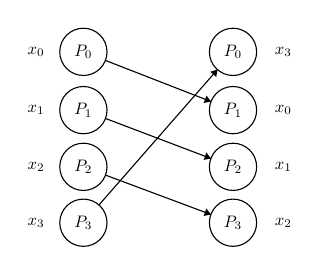
\begin{tikzpicture}[scale=0.1, every node/.style={scale=0.6}]
\tikzstyle{every node}+=[inner sep=0pt]
\draw [black] (26.1,-3.2) circle (3);
\draw (26.1,-3.2) node {$P_0$};
\draw [black] (7.1,-3.2) circle (3);
\draw (7.1,-3.2) node {$P_0$};
\draw [black] (7.1,-17.8) circle (3);
\draw (7.1,-17.8) node {$P_2$};
\draw [black] (7.1,-24.9) circle (3);
\draw (7.1,-24.9) node {$P_3$};
\draw (32.5,-3.2) node {$x_3$};
\draw [black] (26.1,-10.6) circle (3);
\draw (26.1,-10.6) node {$P_1$};
\draw [black] (26.1,-17.8) circle (3);
\draw (26.1,-17.8) node {$P_2$};
\draw [black] (26.1,-24.9) circle (3);
\draw (26.1,-24.9) node {$P_3$};
\draw [black] (7.1,-10.6) circle (3);
\draw (7.1,-10.6) node {$P_1$};
\draw (32.5,-10.6) node {$x_0$};
\draw (32.5,-17.8) node {$x_1$};
\draw (32.5,-24.9) node {$x_2$};
\draw (1.1,-3.2) node {$x_0$};
\draw (1.1,-10.6) node {$x_1$};
\draw (1.1,-17.8) node {$x_2$};
\draw (1.1,-24.9) node {$x_3$};
\draw [black] (9.08,-22.64) -- (24.12,-5.46);
\fill [black] (24.12,-5.46) -- (23.22,-5.73) -- (23.97,-6.39);
\draw [black] (9.9,-4.29) -- (23.3,-9.51);
\fill [black] (23.3,-9.51) -- (22.74,-8.75) -- (22.38,-9.69);
\draw [black] (9.91,-11.66) -- (23.29,-16.74);
\fill [black] (23.29,-16.74) -- (22.72,-15.99) -- (22.37,-16.92);
\draw [black] (9.91,-18.85) -- (23.29,-23.85);
\fill [black] (23.29,-23.85) -- (22.72,-23.1) -- (22.37,-24.04);
\end{tikzpicture}

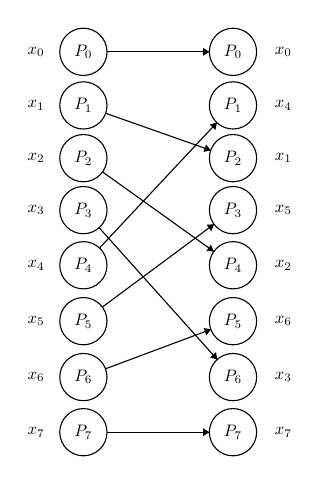
\begin{tikzpicture}[scale=0.1, every node/.style={scale=0.6}]
\tikzstyle{every node}+=[inner sep=0pt]
\draw [black] (26.1,-3.2) circle (3);
\draw (26.1,-3.2) node {$P_0$};
\draw [black] (7.1,-3.2) circle (3);
\draw (7.1,-3.2) node {$P_0$};
\draw [black] (7.1,-16.7) circle (3);
\draw (7.1,-16.7) node {$P_2$};
\draw [black] (7.1,-23.3) circle (3);
\draw (7.1,-23.3) node {$P_3$};
\draw (32.5,-44.5) node {$x_3$};
\draw [black] (26.1,-10) circle (3);
\draw (26.1,-10) node {$P_1$};
\draw [black] (26.1,-16.7) circle (3);
\draw (26.1,-16.7) node {$P_2$};
\draw [black] (26.1,-23.3) circle (3);
\draw (26.1,-23.3) node {$P_3$};
\draw [black] (7.1,-10) circle (3);
\draw (7.1,-10) node {$P_1$};
\draw (32.5,-3.2) node {$x_0$};
\draw (32.5,-16.7) node {$x_1$};
\draw (32.5,-30.3) node {$x_2$};
\draw (1.1,-3.2) node {$x_0$};
\draw (1.1,-10) node {$x_1$};
\draw (1.1,-16.7) node {$x_2$};
\draw (1.1,-23.3) node {$x_3$};
\draw [black] (7.1,-30.3) circle (3);
\draw (7.1,-30.3) node {$P_4$};
\draw [black] (7.1,-37.4) circle (3);
\draw (7.1,-37.4) node {$P_5$};
\draw [black] (7.1,-44.5) circle (3);
\draw (7.1,-44.5) node {$P_6$};
\draw [black] (7.1,-51.5) circle (3);
\draw (7.1,-51.5) node {$P_7$};
\draw [black] (26.1,-30.3) circle (3);
\draw (26.1,-30.3) node {$P_4$};
\draw [black] (26.1,-37.4) circle (3);
\draw (26.1,-37.4) node {$P_5$};
\draw [black] (26.1,-44.5) circle (3);
\draw (26.1,-44.5) node {$P_6$};
\draw [black] (26.1,-51.5) circle (3);
\draw (26.1,-51.5) node {$P_7$};
\draw (32.5,-23.3) node {$x_5$};
\draw (32.5,-37.4) node {$x_6$};
\draw (32.5,-51.5) node {$x_7$};
\draw (32.5,-10) node {$x_4$};
\draw (1.1,-30.3) node {$x_4$};
\draw (1.1,-37.4) node {$x_5$};
\draw (1.1,-44.5) node {$x_6$};
\draw (1.1,-51.5) node {$x_7$};
\draw [black] (10.1,-3.2) -- (23.1,-3.2);
\fill [black] (23.1,-3.2) -- (22.3,-2.7) -- (22.3,-3.7);
\draw [black] (9.93,-11) -- (23.27,-15.7);
\fill [black] (23.27,-15.7) -- (22.68,-14.96) -- (22.35,-15.91);
\draw [black] (9.54,-18.45) -- (23.66,-28.55);
\fill [black] (23.66,-28.55) -- (23.3,-27.68) -- (22.72,-28.49);
\draw [black] (9.1,-25.53) -- (24.1,-42.27);
\fill [black] (24.1,-42.27) -- (23.94,-41.34) -- (23.19,-42);
\draw [black] (9.15,-28.11) -- (24.05,-12.19);
\fill [black] (24.05,-12.19) -- (23.14,-12.43) -- (23.87,-13.12);
\draw [black] (9.51,-35.61) -- (23.69,-25.09);
\fill [black] (23.69,-25.09) -- (22.75,-25.16) -- (23.35,-25.97);
\draw [black] (9.91,-43.45) -- (23.29,-38.45);
\fill [black] (23.29,-38.45) -- (22.37,-38.26) -- (22.72,-39.2);
\draw [black] (10.1,-51.5) -- (23.1,-51.5);
\fill [black] (23.1,-51.5) -- (22.3,-51) -- (22.3,-52);
\end{tikzpicture}

\end{center}
\caption{Permutación por rotación y por baraje-2}
\end{figure}

\textbf{Comunicaciones \textit{compuestas}}

Las comunicaciones compuestas se definen por diferentes modos de reducción de los mensajes enviados por los procesos en los que \textbf{todos combinan} o re realizan por un \textbf{recorrido} (\textit{scan}) paralelo que puede ser \textbf{prefijo} o \textbf{sufijo} en función de si los mensajes se recogen en orden de índice ascendente o descendente respectivamente.

\begin{figure}
\begin{center}
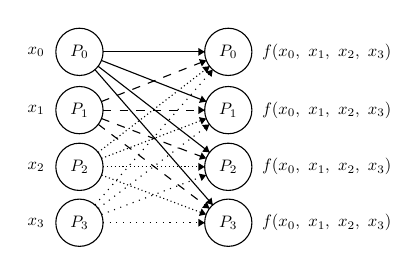
\begin{tikzpicture}[scale=0.1, every node/.style={scale=0.6}]
\tikzstyle{every node}+=[inner sep=0pt]
\draw [black] (25.5,-3.2) circle (3);
\draw (25.5,-3.2) node {$P_0$};
\draw [black] (6.6,-3.2) circle (3);
\draw (6.6,-3.2) node {$P_0$};
\draw [black] (6.6,-17.8) circle (3);
\draw (6.6,-17.8) node {$P_2$};
\draw [black] (6.6,-24.9) circle (3);
\draw (6.6,-24.9) node {$P_3$};
\draw (38,-3.2) node {$f(x_0,\mbox{ }x_1,\mbox{ }x_2,\mbox{ }x_3)$};
\draw [black] (25.5,-10.6) circle (3);
\draw (25.5,-10.6) node {$P_1$};
\draw [black] (25.5,-17.8) circle (3);
\draw (25.5,-17.8) node {$P_2$};
\draw [black] (25.5,-24.9) circle (3);
\draw (25.5,-24.9) node {$P_3$};
\draw [black] (6.6,-10.6) circle (3);
\draw (6.6,-10.6) node {$P_1$};
\draw (38,-10.6) node {$f(x_0,\mbox{ }x_1,\mbox{ }x_2,\mbox{ }x_3)$};
\draw (38,-17.8) node {$f(x_0,\mbox{ }x_1,\mbox{ }x_2,\mbox{ }x_3)$};
\draw (38,-24.9) node {$f(x_0,\mbox{ }x_1,\mbox{ }x_2,\mbox{ }x_3)$};
\draw (1.1,-3.2) node {$x_0$};
\draw (1.1,-10.6) node {$x_1$};
\draw (1.1,-17.8) node {$x_2$};
\draw (1.1,-24.9) node {$x_3$};
\draw [black] (9.6,-3.2) -- (22.5,-3.2);
\fill [black] (22.5,-3.2) -- (21.7,-2.7) -- (21.7,-3.7);
\draw [black] [densely dotted] (8.97,-15.97) -- (23.13,-5.03);
\fill [black] (23.13,-5.03) -- (22.19,-5.13) -- (22.8,-5.92);
\draw [black] [dotted] (8.57,-22.64) -- (23.53,-5.46);
\fill [black] (23.53,-5.46) -- (22.63,-5.74) -- (23.38,-6.39);
\draw [black] (9.39,-4.29) -- (22.71,-9.51);
\fill [black] (22.71,-9.51) -- (22.14,-8.75) -- (21.78,-9.68);
\draw [black] (8.97,-5.03) -- (23.13,-15.97);
\fill [black] (23.13,-15.97) -- (22.8,-15.08) -- (22.19,-15.87);
\draw [black] (8.57,-5.46) -- (23.53,-22.64);
\fill [black] (23.53,-22.64) -- (23.38,-21.71) -- (22.63,-22.36);
\draw [black] [dashed] (9.39,-9.51) -- (22.71,-4.29);
\fill [black] (22.71,-4.29) -- (21.78,-4.12) -- (22.14,-5.05);
\draw [black] [dashed] (9.6,-10.6) -- (22.5,-10.6);
\fill [black] (22.5,-10.6) -- (21.7,-10.1) -- (21.7,-11.1);
\draw [black] [dashed] (9.4,-11.67) -- (22.7,-16.73);
\fill [black] (22.7,-16.73) -- (22.13,-15.98) -- (21.77,-16.91);
\draw [black] [dashed] (8.99,-12.41) -- (23.11,-23.09);
\fill [black] (23.11,-23.09) -- (22.77,-22.21) -- (22.17,-23.01);
\draw [black] [densely dotted] (9.4,-16.73) -- (22.7,-11.67);
\fill [black] (22.7,-11.67) -- (21.77,-11.49) -- (22.13,-12.42);
\draw [black] [densely dotted] (9.6,-17.8) -- (22.5,-17.8);
\fill [black] (22.5,-17.8) -- (21.7,-17.3) -- (21.7,-18.3);
\draw [black] [densely dotted] (9.41,-18.85) -- (22.69,-23.85);
\fill [black] (22.69,-23.85) -- (22.12,-23.1) -- (21.77,-24.03);
\draw [black] [dotted] (8.99,-23.09) -- (23.11,-12.41);
\fill [black] (23.11,-12.41) -- (22.17,-12.49) -- (22.77,-13.29);
\draw [black] [dotted] (9.41,-23.85) -- (22.69,-18.85);
\fill [black] (22.69,-18.85) -- (21.77,-18.67) -- (22.12,-19.6);
\draw [black] [dotted] (9.6,-24.9) -- (22.5,-24.9);
\fill [black] (22.5,-24.9) -- (21.7,-24.4) -- (21.7,-25.4);
\end{tikzpicture}

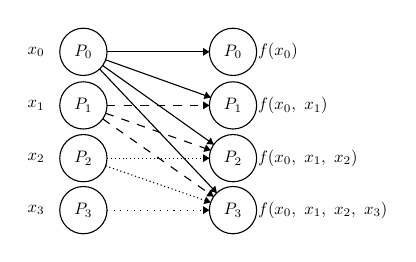
\begin{tikzpicture}[scale=0.1, every node/.style={scale=0.6}]
\tikzstyle{every node}+=[inner sep=0pt]
\draw [black] (26.1,-3.2) circle (3);
\draw (26.1,-3.2) node {$P_0$};
\draw [black] (7.1,-3.2) circle (3);
\draw (7.1,-3.2) node {$P_0$};
\draw [black] (7.1,-16.7) circle (3);
\draw (7.1,-16.7) node {$P_2$};
\draw [black] (7.1,-23.3) circle (3);
\draw (7.1,-23.3) node {$P_3$};
\draw [black] (26.1,-10) circle (3);
\draw (26.1,-10) node {$P_1$};
\draw [black] (26.1,-16.7) circle (3);
\draw (26.1,-16.7) node {$P_2$};
\draw [black] (26.1,-23.3) circle (3);
\draw (26.1,-23.3) node {$P_3$};
\draw [black] (7.1,-10) circle (3);
\draw (7.1,-10) node {$P_1$};
\draw (31.8,-3.2) node {$f(x_0)$};
\draw (35.6,-16.7) node {$f(x_0,\mbox{ }x_1,\mbox{ }x_2)$};
\draw (1.1,-3.2) node {$x_0$};
\draw (1.1,-10) node {$x_1$};
\draw (1.1,-16.7) node {$x_2$};
\draw (1.1,-23.3) node {$x_3$};
\draw (37.5,-23.3) node {$f(x_0,\mbox{ }x_1,\mbox{ }x_2,\mbox{ }x_3)$};
\draw (33.7,-10) node {$f(x_0,\mbox{ }x_1)$};
\draw [black] (10.1,-3.2) -- (23.1,-3.2);
\fill [black] (23.1,-3.2) -- (22.3,-2.7) -- (22.3,-3.7);
\draw [black] (9.92,-4.21) -- (23.28,-8.99);
\fill [black] (23.28,-8.99) -- (22.69,-8.25) -- (22.35,-9.19);
\draw [black] (9.55,-4.94) -- (23.65,-14.96);
\fill [black] (23.65,-14.96) -- (23.29,-14.09) -- (22.71,-14.91);
\draw [black] (9.16,-5.38) -- (24.04,-21.12);
\fill [black] (24.04,-21.12) -- (23.85,-20.2) -- (23.13,-20.88);
\draw [black] [dashed] (10.1,-10) -- (23.1,-10);
\fill [black] (23.1,-10) -- (22.3,-9.5) -- (22.3,-10.5);
\draw [black] [dashed] (9.93,-11) -- (23.27,-15.7);
\fill [black] (23.27,-15.7) -- (22.68,-14.96) -- (22.35,-15.91);
\draw [black] [dashed] (9.56,-11.72) -- (23.64,-21.58);
\fill [black] (23.64,-21.58) -- (23.27,-20.71) -- (22.7,-21.53);
\draw [black] [densely dotted] (10.1,-16.7) -- (23.1,-16.7);
\fill [black] (23.1,-16.7) -- (22.3,-16.2) -- (22.3,-17.2);
\draw [black] [densely dotted] (9.93,-17.68) -- (23.27,-22.32);
\fill [black] (23.27,-22.32) -- (22.67,-21.58) -- (22.35,-22.53);
\draw [black] [dotted] (10.1,-23.3) -- (23.1,-23.3);
\fill [black] (23.1,-23.3) -- (22.3,-22.8) -- (22.3,-23.8);
\end{tikzpicture}

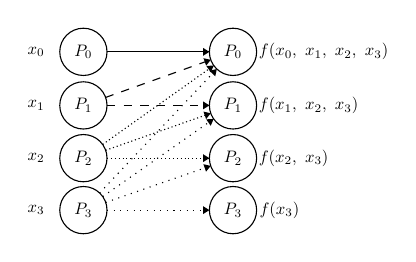
\begin{tikzpicture}[scale=0.1, every node/.style={scale=0.6}]
\tikzstyle{every node}+=[inner sep=0pt]
\draw [black] (26.1,-3.2) circle (3);
\draw (26.1,-3.2) node {$P_0$};
\draw [black] (7.1,-3.2) circle (3);
\draw (7.1,-3.2) node {$P_0$};
\draw [black] (7.1,-16.7) circle (3);
\draw (7.1,-16.7) node {$P_2$};
\draw [black] (7.1,-23.3) circle (3);
\draw (7.1,-23.3) node {$P_3$};
\draw [black] (26.1,-10) circle (3);
\draw (26.1,-10) node {$P_1$};
\draw [black] (26.1,-16.7) circle (3);
\draw (26.1,-16.7) node {$P_2$};
\draw [black] (26.1,-23.3) circle (3);
\draw (26.1,-23.3) node {$P_3$};
\draw [black] (7.1,-10) circle (3);
\draw (7.1,-10) node {$P_1$};
\draw (37.6,-3.2) node {$f(x_0,\mbox{ }x_1,\mbox{ }x_2,\mbox{ }x_3)$};
\draw (33.8,-16.7) node {$f(x_2,\mbox{ }x_3)$};
\draw (1.1,-3.2) node {$x_0$};
\draw (1.1,-10) node {$x_1$};
\draw (1.1,-16.7) node {$x_2$};
\draw (1.1,-23.3) node {$x_3$};
\draw (32,-23.3) node {$f(x_3)$};
\draw (35.7,-10) node {$f(x_1,\mbox{ }x_2,\mbox{ }x_3)$};
\draw [black] (10.1,-3.2) -- (23.1,-3.2);
\fill [black] (23.1,-3.2) -- (22.3,-2.7) -- (22.3,-3.7);
\draw [black] [dashed] (9.92,-8.99) -- (23.28,-4.21);
\fill [black] (23.28,-4.21) -- (22.35,-4.01) -- (22.69,-4.95);
\draw [black] [dashed] (10.1,-10) -- (23.1,-10);
\fill [black] (23.1,-10) -- (22.3,-9.5) -- (22.3,-10.5);
\draw [black] [densely dotted] (9.55,-14.96) -- (23.65,-4.94);
\fill [black] (23.65,-4.94) -- (22.71,-4.99) -- (23.29,-5.81);
\draw [black] [densely dotted] (9.93,-15.7) -- (23.27,-11);
\fill [black] (23.27,-11) -- (22.35,-10.79) -- (22.68,-11.74);
\draw [black] [densely dotted] (10.1,-16.7) -- (23.1,-16.7);
\fill [black] (23.1,-16.7) -- (22.3,-16.2) -- (22.3,-17.2);
\draw [black] [dotted] (9.16,-21.12) -- (24.04,-5.38);
\fill [black] (24.04,-5.38) -- (23.13,-5.62) -- (23.85,-6.3);
\draw [black] [dotted] (9.56,-21.58) -- (23.64,-11.72);
\fill [black] (23.64,-11.72) -- (22.7,-11.77) -- (23.27,-12.59);
\draw [black] [dotted] (9.93,-22.32) -- (23.27,-17.68);
\fill [black] (23.27,-17.68) -- (22.35,-17.47) -- (22.67,-18.42);
\draw [black] [dotted] (10.1,-23.3) -- (23.1,-23.3);
\fill [black] (23.1,-23.3) -- (22.3,-22.8) -- (22.3,-23.8);
\end{tikzpicture}

\end{center}
\caption{Todos combinan, recorrido prefijo paralelo y recorrido sufijo paralelo}
\end{figure}

En OpenMP podemos utilizar las siguientes directivas y cláusulas para crear sistemas de comunicación colectiva:

\begin{center}
\begin{tabular}{l l l}
	\textbf{Servicio} & \textbf{Tipo} & \textbf{Directivas} \\
	\toprule
	\multirow{3}{*}{\textit{uno a todos}} &          & Cláusula \texttt{firstprivate} desde la hebra 0 \\
	                                      & Difusión & Directiva \texttt{single} con cláusula \texttt{copyprivate} \\
	                                      &          & Directiva \texttt{threadprivate} y cláusula \texttt{copyin} en directiva \texttt{parallel} \\
	\midrule
	\textit{todos a uno} & Reducción & Cláusula \texttt{reduction} \\
	\midrule
	\textit{servicios compuestos} & Barreras & Directiva \texttt{barrier}
\end{tabular}
\end{center}

En MPI podemos usar las siguientes funciones:

\begin{center}
\begin{tabular}{l l l}
	\textbf{Servicio} & \textbf{Tipo} & \textbf{Función} \\
	\toprule
	\textit{uno a uno} & Asíncrona & \texttt{MPI\_Send()} o \texttt{MPI\_Receive()} \\
	\midrule
	\multirow{2}{*}{\textit{uno a todos}} & Difusión   & \texttt{MPI\_Bcast()} \\
	                                      & Dispersión & \texttt{MPI\_Scatter()} \\
	\midrule
	\multirow{2}{*}{\textit{todos a uno}} & Reducción   & \texttt{MPI\_Reduce()} \\
	                                      & Acumulación & \texttt{MPI\_Gather()} \\
	\midrule
	\textit{todos a todos} & Todos difunden & \texttt{MPI\_Allgather()} \\
	\midrule
	\multirow{3}{*}{\textit{todos a uno}} & Todos combinan & \texttt{MPI\_Allreduce()} \\
	                                      & Barreras       & \texttt{MPI\_Barrier()} \\
	                                      & Recorrido      & \texttt{MPI\_Scan()} \\
\end{tabular}
\end{center}

\subsection{Paradigmas de programación paralela}\label{paradigmas-progpar}

Dependiendo de la arquitectura con la que estemos trabajando, podemos utilizar diferentes formas de programación paralela:

\subsubsection{Paso de mensajes}

Es el paradigma utilizado en las arquitecturas multicomputador, que necesitan que el computador emisor envíe al receptor los datos con los que necesita trabajar.
Estos sistemas se pueden programar con lenguajes como Ada u Occam y APIs como MPI o PVM\@.

\subsubsection{Variables compartidas}

En los sistemas multiprocesador las variables compartidas pueden alojarse en la memoria compartida y ser accesible por todos los procesadores al mismo tiempo (con sus consecuentes problemas de concurrencia).
Lenguajes como Ada o Java trabajan en este paradigma, así como APIs como OpenMP, Intel TBB (\textit{Threading Building Blocks}) y las hebras POSIX\@.

\subsubsection{Paralelismo de datos}

Es la forma de trabajar de los procesadores matriciales, que requieren una gran potencia de procesamiento.
Se implementa con lenguajes como HPF (\textit{High Performance Fortran}) o Fortran 95, en el que los bloques \texttt{forall} permiten paralelizar operaciones con matrices y vectores, y con APIs como Nvidia CUDA\@.

\subsection{Estructuras típicas de códigos paralelos}\label{estructuras-codigos-paralelos}

\subsubsection{\textit{Maestro-Esclavo} o granja de tareas}

El proceso \textit{maestro} reparte el trabajo a varios procesos \textit{esclavos}\footnote{Es curioso que teniendo el término \textit{granja de tareas} se siga utilizando la notación \textit{Maestro-Esclavo} en lugar de algo más humanitario como \textit{Granjero-Plantación}. El proceso granjero \textit{planta} una serie de subprocesos hijos y espera para cosechar los resultados.}, que realizan su cómputo individualmente y envían el resultado al proceso \textit{maestro} para que éste haga un cómputo final con todos los resultados recolectados.

\subsubsection{Cliente/servidor}

Varios procesos \textit{cliente} mandan peticiones a un proceso \textit{servidor}, que las gestiona y envia respuestas a los procesos \textit{cliente} con el resultado de los cómputos.

\subsubsection{Descomposición de dominio o datos}

Cada proceso adquiere una parte de la computacióna a realizar y entre todos resuelven el problema dividiéndolo en partes equitativas.
Un ejemplo de esto sería el uso de la directiva \texttt{omp for}:

\begin{lstlisting}[language=C]
omp_set_num_threads(hebras)

#pragma omp for
for (int i=0; i<hebras; i++)
	// Acción a realizar individualmente por cada hebra
\end{lstlisting}

\subsubsection{Segmentación o flujo de datos}

Los procesos se organizan de la misma forma que un procesador segmentado de forma que, para cada segmento $i$, éste pueda ejecutarse mientras el resto de segmentos están procesando otra información que llegará al procesador $i$ o de éste.

\subsubsection{Divide y vencerás, descomposición recursiva}

El problema se divide en subproblemas recursivos más pequeños y cada uno de los procesos ejecuta los cómputo de cada uno de los subproblemas.
Cuando dos subproblemas llegan a su caso ancestro común, uno de los procesos se elimina y se continúan los cómputos con el proceso restante.
